\documentclass[twocolumn]{article}

\usepackage{lua-visual-debug}
\usepackage{tikzscale}
\usepackage{tikz}
\usepackage{pgfplots}
\usepackage{currfile}
\usepackage{lmodern}
% Load the MWE package, although its functionality is not needed. The loading highlights, that some graphics used below are part of the MWE package.
\usepackage{mwe}

\usetikzlibrary{external}
\tikzexternalize
% \tikzexternalize[mode=list and make]

\begin{document}
	\section*{Tests}
	\begin{itemize}
		\item Test that with externalization, no picture is generated multiple times.
		\item Test that there are no warnings without using externalization.
		\item Normal input command\\%
			
\begin{tikzpicture}
\draw (0,0) -- (1,1) (0,1) -- (1,0);
\end{tikzpicture}%%
		\item Use includegraphics with file ending\\%
			\includegraphics{testRectangle.tikz}%
		\item Use includegraphics without file ending\\%
			\includegraphics{testRectangle}%
		\item Use includegraphics with scaling to the column's width\\%
			\includegraphics[width=\linewidth]{testRectangle}%
		\item Use includegraphics with scaling to a dimension\\%
			\includegraphics[width=5cm]{testRectangle}%
		\item Use includegraphics with scaling while having column width already\\%
			\includegraphics[width=\linewidth]{linewidth}%
		\item Use includegraphics with jpg\\%
			\includegraphics{example-grid-100x100bp.jpg}%
		\item Use includegraphics with pdf\\%
			\includegraphics{example-grid-100x100bp.pdf}%
		\item Use includegraphics with png\\%
			\includegraphics{example-grid-100x100bp.png}%
% 		\item Use includegraphics with eps%
% 			\includegraphics{example-grid-100x100bp.eps}%
		\item Use includegraphics with pdf and scaling\\%
			\includegraphics[width=0.3\linewidth]{example-grid-100x100bp.pdf}%
		\item Use includegraphics with column width\\%
			\includegraphics[width=\linewidth]{example-grid-100x100bp.jpg}%
		\item Use \texttt{input} with pgfplots\\%
			\begin{tikzpicture}
	\begin{axis}[scale only axis]
		\addplot {x^2 - x + 4};
	\end{axis}
\end{tikzpicture}%
		\item Input a 2D pgfplots\\
			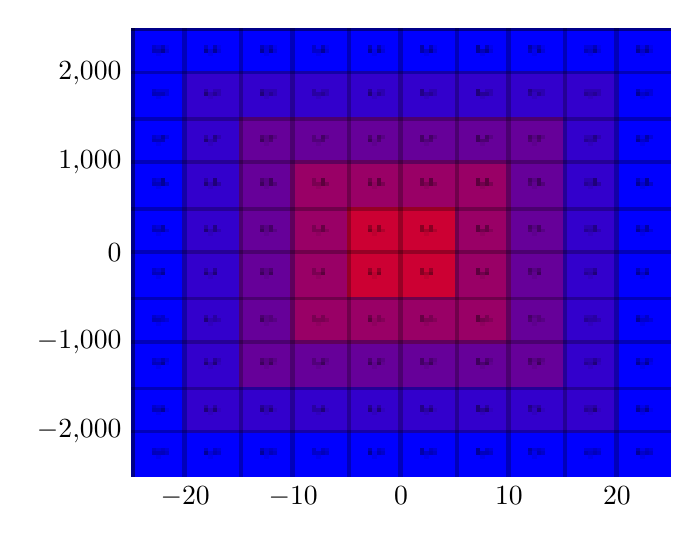
\begin{tikzpicture}
	\begin{axis}[%
		xmin=-25, xmax=25,
		ymin=-2500, ymax=2500]
		\addplot graphics [xmin=-25, xmax=25, ymin=-2500, ymax=2500] {example-grid-100x100bp.png};
	\end{axis}
\end{tikzpicture}%%
		\item Use pgfplots without optional parameter\\%
			\includegraphics{pgfplots-test}%
		\item Use pgfplots with given width and height\\%
			\includegraphics[width=\linewidth,height=0.3\linewidth]{pgfplots-test}%
		\item Use includegraphics with only a node\\%
			\includegraphics{testNode.tikz}%
% 		\item Use includegraphics with scaling only a node results in an error\\%
% 			\includegraphics[width=\linewidth]{testNode.tikz}%
		\item Use includegraphics with a two dimensional plot\\%
			\includegraphics{testgraphic2D.tikz}%
		\item Use includegraphics with a scaled two dimensional plot with line width and an axis ratio of 1\\%
			\includegraphics[width=\linewidth,axisratio=1]{testgraphic2D.tikz}%
		\item Use includegraphics with a scaled two dimensional plot with given height and an axis ratio of 0.5\\%
			\includegraphics[height=\linewidth,axisratio=0.5]{testgraphic2D.tikz}%
		\item Use includegraphics with a scaled two dimensional plot with given height and an axis ratio of 0.5 and temporarily deactivated externalization\\%
			\tikzexternaldisable
			\includegraphics[height=\linewidth,axisratio=0.5]{testgraphic2D.tikz}%
			\tikzexternalenable
		\item Use includegraphics with a scaled two dimensional plot with given height and an axis ratio of 0.5 again\\%
			\includegraphics[height=\linewidth,axisratio=0.5]{testgraphic2D.tikz}%
		\item Use includegraphics with a scaled two dimensional plot with line width and a default axis ratio\\%
			\includegraphics[width=\linewidth]{testgraphic2D.tikz}%
		\item Input a two dimensional plot with a tight frame with width \newlength{\mylen}\settowidth{\mylen}{\frame{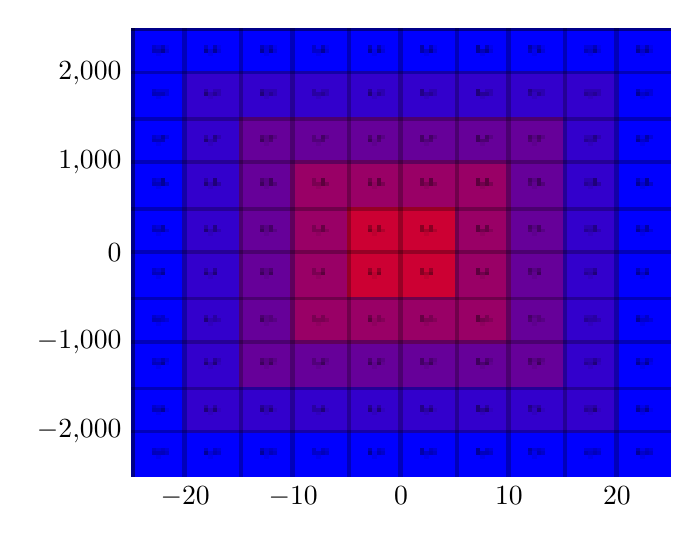
\begin{tikzpicture}
	\begin{axis}[%
		xmin=-25, xmax=25,
		ymin=-2500, ymax=2500]
		\addplot graphics [xmin=-25, xmax=25, ymin=-2500, ymax=2500] {example-grid-100x100bp.png};
	\end{axis}
\end{tikzpicture}%}}\the\mylen\\%
			\frame{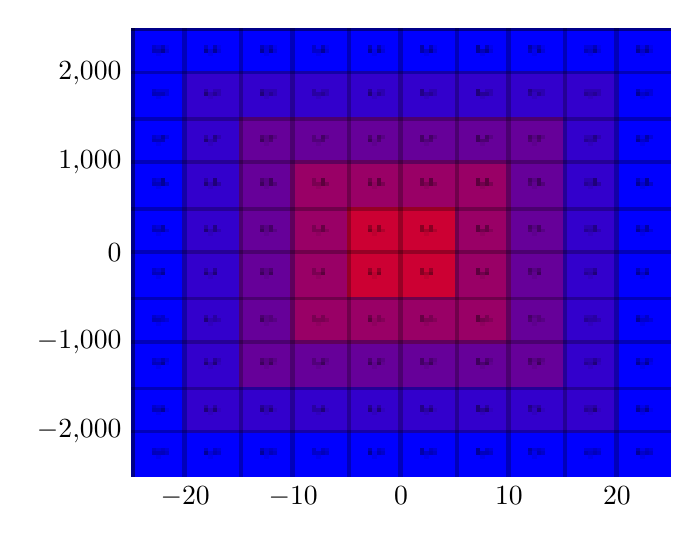
\begin{tikzpicture}
	\begin{axis}[%
		xmin=-25, xmax=25,
		ymin=-2500, ymax=2500]
		\addplot graphics [xmin=-25, xmax=25, ymin=-2500, ymax=2500] {example-grid-100x100bp.png};
	\end{axis}
\end{tikzpicture}%}
		\item Use a two dimensional plot with a tight frame with width \settowidth{\mylen}{\frame{\includegraphics{testgraphic2D.tikz}}}\the\mylen\\%
			\frame{\includegraphics{testgraphic2D.tikz}}
		\item Use includegraphics with a histogram of a normal distribution\\%
			\includegraphics[width=\linewidth,height=0.5\linewidth]{histogramNormal}%
	\end{itemize}
\end{document}